\documentclass[a4paper,10p]{article}
\usepackage[utf8]{inputenc}
\usepackage{graphicx}
\graphicspath{ {BilderTheorie/} }
\usepackage{natbib}
\usepackage{setspace}
\setstretch{1,5}
%\usepackage{ngerman}
\usepackage[a4paper,left=3cm,right=4cm,top=2.5cm,bottom=2cm]{geometry}
\usepackage{setspace}
\setstretch{1,33}
\usepackage[utf8]{inputenc}
\usepackage[ngerman]{babel}
\usepackage{hyperref}
\usepackage{graphicx}
\usepackage{animate}
\usepackage[font={footnotesize}]{subcaption}
\usepackage[font={footnotesize}]{caption}
\DeclareCaptionType{equ}[][]
\usepackage{wrapfig}
\usepackage{amsmath}
\usepackage{movie15}
\usepackage{pdfpages}
\usepackage{natbib}
\usepackage{booktabs}

\setlength{\abovecaptionskip}{5pt}
\setlength{\belowcaptionskip}{-7pt}


%opening
\title{Gattungszuordnung anhand inhaltlicher Merkmale mit Hilfe gängiger stilometrischer Methoden}
\author{Teresa Kaiser, Pia Henning}

\begin{document}
\maketitle
\tableofcontents
\newpage
\listoffigures
\newpage
\section{Einleitung}
Stilometrische Verfahren sind ein gängiges Mittel in der computergestützten Literaturwissenschaft. Obwohl sie für verschiedene Forschungsfragen geeignet sind, werden sie meist für die Autorschaftsattribution eingesetzt. So konnte beispielsweise die Autorschaft von J. K. Rowling, bei dem unter Pseudonym veröffentlichten Roman \emph{The Cuckoo's Calling}, nachgewiesen werden. Auch vor Gericht haben stilometrische Analysen Gewicht, wie bei der Asylverhandlung von \glqq Bilbo Baggins\grqq \citep{Juola2015}.

Die Autorschaftsattribution mit Hilfe stilometrischer Methoden anhand inhaltlicher Merkmale generiert zuverlässige Ergebnisse, da Störvariablen wie Gattung, Genre, Epoche, Alter und Geschlecht des Autors bei der Korpuserstellung herausgefiltert werden. Während hier viele Forschungsergebnisse vorliegen, ist die stilometrische Zuordnung zu Gattungen, Genre etc. kaum erforscht. Bei ent\-sprech\-en\-dem Korpusaufbau sollte dies allerdings gleichermaßen durchführbar sein. Da die Zuordnung zu Gattungen als Basiskategorisierung literarischer Texte gilt, untersucht die vorliegende Arbeit die computergestützte Unterscheidung nach Gattungszugehörigkeit. 

Es wird davon ausgegangen, dass lyrische und epische Texte anhand ihrer quantifizierbaren, inhaltlichen Merkmale voneinander abgrenzbar sind. Da hierzu kaum Forschungsarbeiten zugänglich sind, soll die stilometrische Analyse der Gattungszuordnung mit den Basisverfahren Zeta und Delta durchgeführt werden, um eine Grundlage für die weitere Forschung zu schaffen. Diese Methoden sind zudem interessant, da sie die Texte mit unterschiedlicher Herangehensweise auf Wortebene untersuchen. So betrachtet das Zeta die Eindeutigkeit der verwendeten Wörter nach Korpus, während das Delta die Zuordnung der einzelnen Texte anhand der häufigsten Wörter vornimmt. 

Nach der Datenexploration sowie den theoretischen Grundlagen folgt die erste Anwendung der vorgestellten Methoden. Anhand dieser Ergebnisse wird die Fragestellung verfeinert und der Versuchsaufbau ausgeweitet.

FRAGE:   Lassen sich Gedichte und Prosa Texte stilometrisch nach ihren inhaltlichen Gattungsmerkmalen unterscheiden? Können Störsignale/ Noise aus Autorschaft/ Zeit etc. eliminiert werden?


\section{ Datenexploration}

Um zuverlässige Ergebnisse erzielen zu können und Zufälligkeiten in den Beobachtungen auszuschließen, werden die Analysen in dieser Arbeit mit mehreren unterschiedlich zusammengesetzten Korpora durchgeführt. Beim Aufbau der Korpora wurde darauf geachtet, so viel Noise wie möglich zu reduzieren. So stammen alle Texte aus dem 19. Jahrhundert, sind also einer ähnlichen Epoche zuzuordnen. Um das Rauschen von geschlechterspezifischem Stil zu minimieren, sind zudem Texte sowohl von weiblichen als auch von männlichen Autoren enthalten. Störsignale, die auf Gattung und Genre zurückzuführen sind, nehmen für die vorliegende Forschungsfrage eine besondere Position ein, da sie im Fokus liegen. Um Lyrik und Epik gegenüberstellen und voneinander trennen zu können, wurde deshalb darauf geachtet, für jedes Korpus eine annähernd vergleichbare Anzahl an Tokens pro Gattung ohne Stopwörter zu verwenden. Einige Noise-Quellen werden so also reduziert. Eine Herausforderung stellt allerdings noch das Rauschen des Autorsignals dar. Der Umgang damit, beim Aufbau der Korpora, wird im Folgenden mit Blick auf die spezifischen Eigenschaften ausgeführt. Der exakte Aufbau der vier verwendeten Textsammlungen ist in Abbildung \ref{fig:Zusammenstellung_Korpora} dargestellt.


\begin{figure}[h]
	\begin{center}
	\resizebox{\textwidth}{!}{
	\begin{tabular}{@{}lllllll@{}}
				\toprule
		Korpus           & Anzahl Epik & Anzahl Lyrik & Gesamt & Anzahl Autoren & Tokens  & Anzahl Segmente500 \\ \midrule
		Hauptkorpus      & 22          & 4.748         & 4.770   & 948            & 1.621.344 & 1.384               \\
		Autorenkorpus    & 6           & 2.418         & 2.424   & 6              & 3.585.102 & 644                \\
		Vergleichskorpus & 6           & 2.418         & 2.424   & 713            & 930.024  & 616/ 674           \\
		Fontanekorpus    & 1           & 750          & 751    & 1              & 285.959  & 246              \\ \bottomrule  
	\end{tabular}}
\end{center}
\caption{Zusammenstellung der Korpora}
\label{fig:Zusammenstellung_Korpora}
\end{figure}


Das Hauptkorpus wird verwendet, um erste Ergebnisse zu generieren und eine Einschätz\-ung für die entstehenden Werte und ihr Zusammenspiel mit der Zusammensetzung des Korpus zu erlangen. Um eine annähernd ausgeglichene Tokenanzahl zwischen Epik und Lyrik zu erreichen, werden 22 Romane und 4.748 Gedichte verwendet. Die Quelle der epischen Texte ist \citep{ComputationalStylisticsGroup}, der aus 68 Texten von 22 Autoren aufgebaut ist. Hieraus wurden für das Hauptkorpus je ein Roman pro Autor randomisiert ausgewählt. Die Gedichte stammen aus dem DFG-Projekt \textit{Die Anfänge der modernen Lyrik - Literaturgeschichte mit Textähnlichkeiten modellieren} \footnote{Es handelt sich dabei um ein laufendes, noch unveröffentlichtes Projekt der Julius-Maximilians-Universität Würzburg und der Georg-August-Universität Göttingen unter Leitung der Professoren Jannidis und Winko. Für die vorliegende Arbeit wurde das Korpus (Stand 1.Juli 2020) verwendet.}. Aus diesem Korpus werden die Texte aller 18 unbalanciert aufgebauter Anthologien verwendet, die von insgesamt 926 Autoren verfasst sind. \par 

Für die Berechnung des Zeta werden daraus für jede Gattung Segmente einer bestimmten Länge erstellt, in diesem Fall mit 500 Tokens pro Segment. Trotz der unterschiedlichen Anzahl der Dokumente bei Epik und Lyrik entsteht daraus eine ähnliche Zahl an Segmenten. Um diese Anzahl exakt anzugleichen, werden die überschüssigen Segmente randomisiert heraus gesamplet, was zu einem finalen Wert von je 1384 Segmenten führt. Der starke Unterschied der Textlängen von Epik und Lyrik wird so zumindest etwas reduziert. Auch bei der Delta-Analyse stellt diese Varianz zumindest grundlegend kein Problem dar, da aufgrund der Verwendung des Cosinus-Deltas die Distanz zwischen zwei Textvektoren nicht auf Basis deren Länge, sondern des Winkels zwischen ihnen berechnet wird. Diese Problematik soll im Kapitel zum Delta weiter unten eingehender diskutiert werden. \par 

Da davon ausgegangen werden muss, dass das Autorensignal einen starken Einfluss auf die Ergebnisse haben kann, wurde beim zweiten Korpus, dem Autorenkorpus, versucht, dieses Rauschen zu regulieren. Die Textsammlung enthält mit sechs Urhebern deutlich weniger unterschiedliche Schriftsteller als das Hauptkorpus \footnote{Die Epiktexte wurden aus dem Korpus der European Literary Text Collection \citep{ELTEC} verwendet, die Lyriktexte wurden von Textgrid \citep{textgrid} gescraped}. Alle Autoren sind sowohl in der Epik als auch in der Lyrik vertreten, anders als vorher, wo es in dieser Hinsicht keine Überschneidungen gab. Zudem handelt es sich ausschließlich um Autoren, die im Hauptkorpus nicht vertreten sind. Damit ergibt sich nicht nur die Möglichkeit, die Attributionswerte von zwei komplett unterschiedlichen Korpora gegenüber zu stellen. Auf diese Weise wird auch das Autorschaftssignal weiter untersucht. Im Hauptkorpus verteilen sich die Texte einerseits auf eine sehr große Anzahl unterschiedlicher Urheber, was einerseits darauf hinweisen kann, dass sich die individuellen Stile verflüchtigen, andererseits aber auch bedeuten kann, dass einzelne Autoren, die häufiger als andere vertreten sind, die Suche nach gattungsspezifischen Merkmalen mit ihrem eigenen Stil verfälschen. Deshalb wird mit dem Autorenkorpus versucht, einen so weit wie möglich balancierten Aufbau zu erlangen. \par 

Manche Autoren, wie Fontane oder Keller, haben deutlich mehr Gedichte verfasst als andere, weshalb der Anteil ihrer Texte pro Gattung, was die Tokenanzahl betrifft, recht ausgeglichen ist. Die Analysen werden zeigen, ob der dadurch entstehende, etwas unregelmäßige Aufbau einen Einfluss auf die Ergebnisse hat. Mit Hinblick auf das Autorschaftssignal wird davon ausgegangen, dass durch das Vorkommen der Autoren in beiden Gattungen verhindert wird, dass ein Schriftsteller mit seinem individuellen Stil beispielsweise den Stil der Epik allgemein signifikant beeinflusst. Stattdessen tritt das Autorenrauschen dadurch in beiden Gattungen auf und führt somit, so die Hypothese, zu einer Art Noise, der in Epik und in Lyrik in ungefähr gleichmäßig auftritt und somit das Gesamtergebnis im Durchschnitt nicht verfälschend beeinflusst. \par 

Um das Rauschen des Autorsignals noch weiter zu beobachten und eine Möglichkeit zu finden, es zu messen, werden die Analysen schließlich mit den verbleibenden beiden Korpora durchgeführt. Das Vergleichskorpus ist aus dem Hauptkorpus gesamplet und enthält damit ebenfalls eine recht hohe Anzahl an Autoren. Es wird im Zusammenspiel mit dem Fontanekorpus analysiert, das lediglich die Texte von Fontane aus dem Autorenkorpus enthält. Dadurch entsteht der Versuch, die beiden oben vorgestellten Ansätze des Korpusaufbaus zu vereinen. Die Berechnungen werden mit vier unterschiedlichen Zusammensetzungen durchgeführt, womit versucht wird zu beobachten, ob und inwieweit das teilweise oder komplette Hinzufügen der Fontanetexte einen Einfluss auf die Ergebnisse nimmt. Zudem verfügt das Vergleichskorpus mit 6 Epik- und 2418 Lyriktexten über das gleiche Verhältnis an Dokumenten pro Gattung wie das Autorenkorpus. Durch die Varianz der Länge von Epiktexten, enthält das Autorenkorpus deutlich mehr Tokens. Da aber die Anzahl der Segmente jeweils an die Lyrik angepasst wird, entstehen am Ende sowohl für das Vergleichs als auch für das Autorenkorpus ähnlich viele Segmente. Die Anzahl der Segmente im Vergleichskorpus wird zudem erst in Zusammensetzung mit dem Fontanekorpus angepasst, weshalb an dieser Stelle im Abbildung \ref{fig:Zusammenstellung_Korpora} zwei Werte aufgeführt sind. \par

\begin{wrapfigure}{l}{0.5\textwidth}
	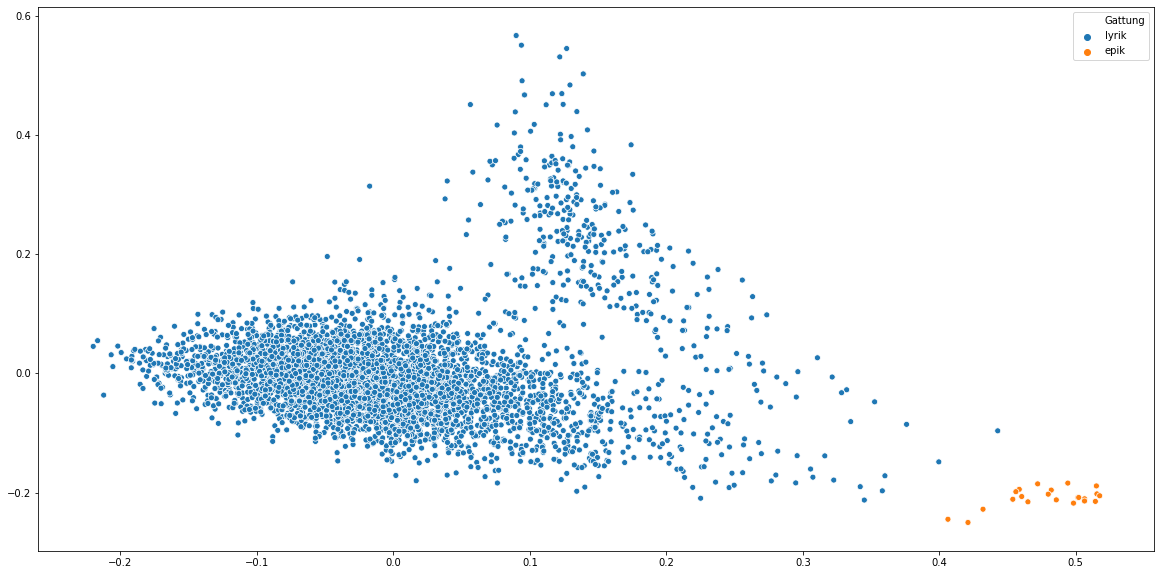
\includegraphics[width=0.5\textwidth]{pca_mfw.png}
	\caption{PCA mit den 1000 most frequent words des Hauptkorpus}
	\label{fig:PCA_mfw}
\end{wrapfigure}

Ein Blick auf die rohen Textdaten gibt einen ersten Anhaltspunkt, der die Hypothese, dass Epik und Lyrik auf Ebene der Inhaltswörter voneinander abgrenzbar sind, unterstützt. Mithilfe einer PCA werden in Abbildung \ref{fig:PCA_mfw} die 1000 häufigsten Wörter im Hauptkorpus auf zwei Hauptkomponenten reduziert. Die orangen Datenpunkte, die für Epik stehen, grenzen sich allein anhand dieser räumlichen Darstellung der Features recht deutlich ab. Anhand dieses ersten Anhaltspunktes ergibt sich die Nachforschung zu weiteren inhaltlichen Merkmalen, die die beiden Gattungen individuell identifizierbar machen. Eine Überlegung führt zur Emotionalität, die in den Texten ausgedrückt wird und die besonders Gedichte auszeichnet. Um diese Annahme zu verfolgen, bietet es sich an die Korpora mithilfe des Tools SENTTEXT zu analysiern. ERGEBNISSE Die Liste der Emotionen von \textit{SentiWS} \citep{Sentiws} ist stark von Polarität geprägt und beinhaltet besonders auch Wörter, die den impliziten Ausdruck von Gefühl betonen. \par 

Die Analyse zeigt, dass für die Distinktivität von Lyrik aber eher explizite Emotionswörter geeignet sind. Deshalb dient die Analyse mit \textit{SentText} zunächst nur als Bestätigung, dass bestimmte Merkmale spezifisch für eine Gattung stehen können. Die exakten Features, die für die stilometrischen Analysen verwendet werden sollen, werden daher aber erst im Folgenden ausgewählt, nachdem die Gattungen Epik und Lyrik beleuchtet wurden.\par 


NOTIZEN:
Lyrik vs. Epik: Tokenzahl/ type-token-ratio (mehr Wörter = größere Varianz? --> kleinere Zetawerte?)

Senttext --> häufigste Wörter pro Genre etc --> Wordcloud
-> Prosa implizierter, Lyrik explizit. Deshalb SenText nicht aussagekräftig.

SenText Ergebnis: Ausgewogene Verteilung(positiv und negativ) sowohl mit BAWL als auch der SentiWS Liste. Aber bei Wordcloud: Unterschiedliche Wörter -> Gedichte haben mehr reine Emotionswörter und Emotionstags.
Liste der Emotionslklassifikation (HiWi) -> davon Emotionswörter
uns ist Polarität egal, hauptsache Emotion


\section{Gattungsmerkmale}
Die deutsche Literatur wird üblicherweise in die drei Hauptgattungen Epik, Drama und Lyrik untergliedert. Sie lassen sich anhand zahlreicher Merkmale klar abgrenzen. Literaturwissenschaftlich, mit Hilfe von stilometrischen Methoden, am besten untersucht sind Prosatexte der Gattungen Epik und Drama. Um nun erforschen zu können, ob sich lyrische Texte des 19. Jahrhunderts mit den gleichen stilometrischen Vorgehensweisen untersuchen lassen, wurde ein episches Vergleichskorpus gewählt, um Rauschen durch Szenenbeschreibungen auszuschließen. \par 

Um ein möglichst aussagekräftiges Ergebnis erhalten zu können, werden die Parameter der Berechnungen und die zu vergleichenden Merkmale an die Abweichungen der jeweiligen Gattungsmerkmale angepasst. \par 

Lyrische Texte sind Verstexte, die nicht episch oder dramatisch sind. Üblicherweise sind sie in Versform verfasst und bilden vom Satz unabhängige Einheiten. Sie sind monologisch, statt dialogisch aufgebaut, dadurch werden keine Gesprächssituationen gebildet. Als einzige Ausnahme fungieren Balladen, die als einzige lyrische Form direkte Rede beinhalten. Lyrik bedient sich stattdessen vermehrt an Metaphern, Symbolen, Allegorien und Metonymien. Rein formal betrachtet unterscheiden sich lyrische Texte insbesondere durch den Textumfang und die metrische Form der Verse und somit die gebundene Form der Sprache, die in Wort-und Satzakzent über die Normalsprache hinausgeht \citep[vgl.][S. 111]{Krah2006}. Als wichtigstes lyrisches Kriterium gilt jedoch die Leidenschaft und Emotion der Texte \citep[vgl.][S. 462-464]{SchweikleGunther;Burdorf2007}. \par 

Eine Schwierigkeit bei der Definition von lyrischen Merkmalen ist die Vielzahl der Gedichtformen, die jeweils starke eigene Merkmale aufweisen \citep[vgl.][S. 119]{Krah2006}. \par 

Epische Texte zeichnen sich im Gegensatz dazu durch die Erzählinstanz und Erzählgegenstand aus. Sie werden der erzählenden Literatur zugeordnet und können sowohl in Prosa als auch in Versform verfasst sein. Auch der Umfang ist nicht ausschlaggebend \citep[vgl.][S. 195]{SchweikleGunther;Burdorf2007}. \par 

Da nicht nur Gattungen, sondern auch die literaturwissenschaftlichen Epochen und Strömungen Gemeinsamkeiten und Merkmale aufweisen \citep[vgl.][S. 274]{Krah2006}, werden zur Analyse die Korpora mit Texten der gleichen Zeitspanne aufgebaut. Hierfür wurde das 19. Jahrhundert gewählt, da zu dieser Zeit die gängige Einteilung der Gattungen kanonisiert wurde \citep[vgl.][S. 368]{Krah2006}.


\section{Exkurs}
\subsection{Emotionen und Emotionsklassifikation}
Beim Hauptmerkmal der Lyrik auf inhaltlicher Ebene handelt es sich um Emotionen. Hierbei wichtig ist die Begriffsklärung der Emotion und Auseinandersetzung mit der sprachlichen Darstellung. Da Emotionen unseren Alltag, Handeln und den zwischenmenschlichen Umgang prägen, besitzt jeder eine Vorstellung von Emotion, dennoch fällt das Erkennen und Ausdrücken häufig schwer. Es handelt sich um ein komplexes Zusammenspiel subjektiver und objektiver Faktoren, mit Auswirkungen auf unser neuronales System \citep[vgl.][S. 355]{KleinginnaPaulR;Kleinginna1981}. Dies erschwert die Untersuchung und klare Definition des Emotionsbegriffs. \par 

\begin{wrapfigure}{l}{0.5\textwidth}
	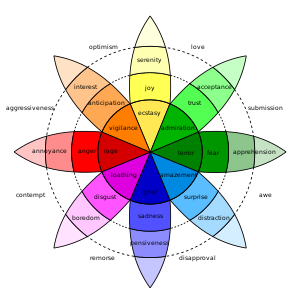
\includegraphics[width=0.5\textwidth]{plutchik_wheel.png}
	\caption{Plutchiks Wheel of Emotions}
	\label{Wheel}
\end{wrapfigure}

Eine Minimaldefinition erleichtert die Herangehensweise und Untersuchung. Das automatisierte Erkennen von Emotionen fällt bei expliziten Emotionen wesentlich leichter, da hier die Emotion durch ein prototypisches Emotionswort explizit thematisiert wird \citep[vgl.][S. 34-41; S. 76-84]{Hillebrandt2011}. \par 


Die Vielzahl an Emotionen wurden im Laufe der Zeit von verschiedenen Wissenschaftlern aus diversen Disziplinen klassifiziert. Eines der bekannten Klassifikationssysteme stammt von Robert Plutchik, der die Emotionen in einem Rad der Emotionen zusammenfasst. Er benennt acht Primäremotionen (\textit{Wut}, \textit{Ekel}, \textit{Trauer}, \textit{Begeisterung}, \textit{Panik}, \textit{Erwartung}, \textit{Überraschung}, \textit{Vertrauen}), die in zwei weiteren Etappen abgestuft werden, wobei die Intensität der Emotionen kontinuierlich abnimmt. Ähnliche Emotionen sind in Plutchiks Darstellung benachbart \citep[vgl.][S. 40-122]{Plutchik}. 

\begin{wrapfigure}{r}{0.5\textwidth}
	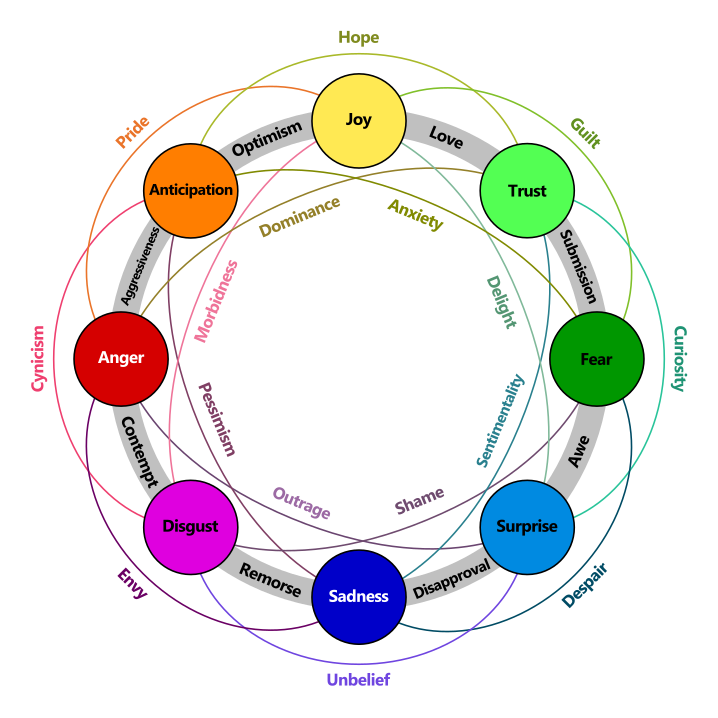
\includegraphics[width=0.5\textwidth]{Plutchik_Dyads.png}
	\caption{Plutchiks Übersicht zu Dyaden der Emotionen}
	\label{fig:Dyads}
\end{wrapfigure}

Neben den primären Emotionen hat Plutchik auch primäre, sekundäre und tertiäre Emotionspaare definiert, wobei die Emotion eines primären Emotionspaars aus zwei direkt benachbarten Emotionen gebildet wird, sekundäre Emotionspaare aus zwei Feldern entfernten Emotionen besteht und tertiäre Emotionspaare drei Felder voneinander entfernt sind. Vier Felder entfernte und somit gegensätzliche Emotionen sind gegenteilige Emotionspaare \citep[vgl.][S. 40-122]{Plutchik}.\par 

Das Ziel Plutchiks Konzepts ist es, alle evolutionären Level der Emotionen aller Tiere, inklusive Menschen, abzubilden und diese Emotionen als Grundlage zur Bildung weiterer Emotionen darzustellen. Das Modell ist für die Analyse von Emotionen in der Literatur geeignet, da es die wichtigsten und somit stärksten Emotionen abbildet \citep[vgl.][S. 40-122]{Plutchik}. \par 

Aus diesem Grund werden für die nachfolgende Analyse der Emotionen in Lyrik und Epik die acht Basisemotionen Wut, Ekel, Trauer, Begeisterung, Panik, Erwartung, Überraschung, Vertrauen als Emotionswörter herangezogen. Der Liste der Emotionswörter VERLINKEN wird zusätzliche ihre adjektivische und gegebenenfalls verbale Verwendung hinzugefügt, sowie die Emotion \textit{Liebe}, da sie durch Liebeslyrik und Liebesromane bezeichnend und namensgebend sowohl für Epik, als auch Lyrik ist. 
 

\subsection{Direkte Rede}
Ein auszeichnendes Merkmal von epischen Texten, das sie zudem von Gedichten abgrenzt, ist die Darstellung der Kommunikationssituation. Sie beinhalten immer eine Erzählerfigur, die Hintergrundwissen liefert und von Geschehnis zu Geschehnis führt \citep[vgl.][S. 9]{Bloß2005}. Dabei wird den handelnden Charakteren entweder die Möglichkeit gegeben, sich selbst in Form einer direkten Rede auszudrücken, oder sie werden durch den Erzähler indirekt zitiert. Letzteres ist ebenso wie die Erzählsituation, ob auktorial oder personal, aber nur schwer quantifizierbar, da diese Merkmale sich stark auf inhaltlicher und syntaktischer Ebene befinden. Aus diesem Grund ist die direkte Rede für die vorliegende Analyse am interessantesten.\par 

Hierbei stechen zwei Merkmale besonders heraus: die Absetzung der Aussage vom restlichen Text durch Satzzeichen sowie die Einleitung der Aussage durch ein sogenanntes "verbum dicendi" \citep[S. 6]{Bloß2005}. Beide bieten sich sehr gut für die Verwendung in stilometrischen Verfahren an. Die Absetzung der Rede kann durch Interpunktionszeichen wie Punkt, Komma, Anführungszeichen und Gedankenstriche beobachtet werden. Da Punkte und Kommata mehrdeutig sind und Gedankenstriche auch in der Lyrik ohne Zusammenhang zu direkter Rede verwendet werden, sind Anführungszeichen für diesen Fall die beste Wahl \citep[vgl.][S. 34]{Bloß2005}.\par 

Das zweite hilfreiche Merkmal, die redeeinleitenden Verben, bieten sich ebenfalls für die rechnerische Analyse von Texten an, indem eine Liste davon mit den Dokumenten abgeglichen werden kann. Literaturwissenschaftlich wurde festgestellt, dass das beliebteste verbum dicendi \textit{sagen} ist. Die Spannweite der möglichen Verben ist aber deutlich größer. Während \textit{sagen} als Verb ohne bestimmte Merkmale zur Artikulationsart gilt, gibt es beispielsweise auch Verben, durch die sie Kommunikationssituationen gliedern lassen, wie \textit{fragen} oder \textit{unterbrechen}, die die Sprechabsicht definieren wie \textit{behaupten} oder \textit{vorschlagen} oder die die Aussage lautlich beschreiben wie \textit{flüstern} oder \textit{singen} \citep[vgl.][S. 66-68]{Bloß2005}. Bei der Erstellung einer Referenzliste mit redeeinleitenden Verben sollte deshalb darauf geachtet werden, diese verschiedenen Abstufungen zu berücksichtigen, um die Variabilität über unterschiedliche Texte in die jeweilige Analyse miteinbeziehen zu können.


\section{Zeta}
Um die beiden Korpora auf sprachlicher und literaturwissenschaftlicher Ebene untersuchen zu können, wird im folgenden Textabschnitt eine kontrastierende Analyse, mit Hilfe eines Zeta-Maßes, durchgeführt, um zu testen, ob die formalen Unterschiede der Gattungen wie oben definiert auf das vorliegende Korpus zutreffen. Ursprünglich wurde das Maß von John Burrow vorgeschlagen, Christof Schöch zeigt anhand einer neuen Implementierung dessen Möglichkeiten bei der Unterscheidung der drei dramatischen Gattungen Komödie, Tragödie und Tragikomödie auf \citep[vgl.][S. 77 f.]{SchöchZeta}. \par 

Da es laut  Schöch \glqq mathematisch gut nachvollziehbar\grqq \footnote{\citep[S. 78]{SchöchZeta}} ist und seine Ergebnisse gut interpretierbar sind, ist davon auszugehen, dass es für die erste Analyse der Gattungsunterschiede zwischen Lyrik und Epik, geeignet ist, da es sich ebenfalls um klar abgrenzbare Gattungen handelt.\par 

Bei dem Zeta-Maß handelt es sich um ein Maß für Distinktivität, der sogenannten \glq keyness \grq, von Merkmalen. Es eignet sich daher gut für eine binäre Klassifikation von Texten. Für die Differenzierung von Lyrik und Epik auf Textebene anhand charakteristischer Merkmale werden im Folgenden Emotionen und direkte Rede untersucht. \par 

Aufgrund der zuvor ermittelten Gattungsmerkmale, ist davon auszugehen, dass die Emotionen, Emotionswörter und Emotionstagger, wie beispielsweise \textit{fühlen}, charakteristisch dem Lyrik-Korpus zugesprochen werden können, wohingegen Merkmale der direkte Rede, wie Anführungszeichen und Verben der direkten Rede, charakteristisch dem Epik-Korpus zugeordnet werden können. \par 

Die charakteristische Zuordnung wird durch das Verhältnis der relative Häufigkeiten des Merkmals in beiden Partitionen ermittelt (\textit{rff}). Dafür wird für jedes Merkmal \textit{i} die relative Häufigkeit \textit{rf} in der Zielpartition \textit{Z} und der Vergleichspartition \textit{V} ermittelt. Die \textit{rf} der Zielpartition durch den Wert der Vergleichspartition dividiert \citep[vgl.][S. 79 f.]{SchöchZeta}.\\



\begin{align}
rrf_{i}=\frac{rf_{i}(Z)}{rf_{i}(V)}
\end{align}
\\

Für die Analyse durch das Zeta-Maß, werden beide Partitionen in gleich lange Segmente aufgeteilt. Wodurch eine Untersuchung sowohl von langen als auch kurzen Texten möglich ist. Es folgt keine Erhebung der Häufigkeit eines Merkmals pro Segment, sondern die Anzahl der Segmente, in denen das Merkmal mindestens einmal vorkommt. Der resultierende Wert gibt an, wie konsistent das Merkmal in den unterschiedlichen Partitionen Verwendung findet \citep[vgl.][S. 79 f.]{SchöchZeta}.\\


\begin{equ}[h]
		\begin{equation}
	dp_{i}(Z)=\frac{df_{i}(Z)}{n(Z)} \qquad  \mathrm{ bzw.} \qquad  dp_{i}(V)=\frac{df_{i}(V)}{n(V)}
	\end{equation}
\end{equ}


Dafür wird jedes Merkmal \textit{i} erhoben in wie vielen Segmenten von \textit{Z} und \textit{V} es jeweils vorkommt (\textit{df}). Diese Werte werden zu Anteilen umgerechnet (\textit{n(Z)},\textit{n(V)}). Die Zeta-Formel erhält man durch Subtraktion des Anteils der Zielpartition mit dem Anteil der Vergleichspartition \citep[vgl.][S. 79 f.]{SchöchZeta}.\\

	\begin{equ}
		\begin{equation}
		Zeta_{i}=dp_{i}(Z)-dp_{i}(V)
		\end{equation}
	\end{equ}
	 
 
Der Zeta-Wert liegt zwischen -1 und 1. Tendiert er gegen 1, ist das Merkmal für die Zielpartition besonders charakteristisch, tendiert er gegen -1 ist er äußerst uncharakteristisch für die Zielpartition. Bei einer Tendenz gegen 0, kommt das Merkmal in jedem Segment beider Partitionen gleich oft vor \citep[vgl.][S. 79 f.]{SchöchZeta}.

Für die vorliegende Analyse der Gattungsmerkmale wurden spezifische Listen gewählt. Für die Sprechmarker wurden Dornseiff \citep{Dornseiff2000} und Bloß \cite{Bloß2005} als Quellen herangezogen und miteinander abgeglichen. Für die Untersuchung der Emotionen liegt die Liste von Plutchiks Emotionen inklusive \textit{Liebe} \citep{Plutchik}, sowie ihre Erweiterung durch Adjektive und Verben und \textit{SentiWS} \citep{Sentiws} vor.

\section{Delta}
Als weiteres stilometrisches Verfahren zur Unterscheidung epischer und lyrischer Texte wird das von Burrows entwickelte Deltamaß getestet. Da es sich in verschiedensten Anwendungsfällen als zuverlässiges, robustes Maß erwiesen hat, das häufig für erste Baseline-Ergebnisse verwendet wird und zudem von Burrows als geeignet für die stilometrische Analyse von Gattungen vorgestellt wurde, wird es auch für die vorliegende Arbeit verwendet, um die formulierte Hypothese zusätzlich zu testen.\par 

Die Grundidee des Delta ist es, den Mittelwert der absoluten Differenzen zwischen den Z-Scores für alle betrachteten Wörter der beiden verglichenen Texte zu berechnen \citep[vgl.][S. 17]{Stamatatos}. Je kleiner der berechnete Delta-Wert zwischen zwei Texten ist, desto größer ist die stilistische Ähnlichkeit zwischen ihnen einzustufen. Da die große Anzahl von einmalig auftretenden Wörtern Überlegungen verlangsamt und erschwert, wird nur eine vorher festgelegte Menge von häufigsten Wörtern verwendet, die nach der Berechnung der Z-Scores abgeschnitten wird. Aufgrund der Heterogenität der Textsammlung, die zwischen sehr langen Romantexten und teils sehr kurzen Gedichten schwankt, werden Analysen mit 1000 most frequent words (MFW) durchgeführt, da dies nicht nur ein allgemein häufig gewählter Wert für das Delta ist, sondern auch ein ungefähres Mittel darstellt, das beide Textsorten berücksichtigt. Zudem wird in einem weiteren Versuch getestet, wie sich die für das Zeta erstellten Segmente mit je 500 Tokens verhalten. \par 

Für die folgenden Berechnungen soll im Speziellen das Cosinus-Delta angewandt werden, das die Distanz zwischen zwei Dokumentvektoren mithilfe des Winkels zwischen ihnen misst. Da hierbei die Länge der einzelnen Texte an Bedeutung verliert, ist diese Version für die Analyse von Texten unterschiedlicher Gattungen und damit auch stark variierender Länge besser geeignet als Deltaverfahren, die z.B. die Manhattan- oder die Euklidische Distanz berechnen \citep[vgl.][S. ii9]{Evert2017a}.\par 

Die Berechnung des Cosinus-Deltas basiert auf folgender Formel \citep[vgl.][S. ii6]{Evert2017a}, die mit den Z-Scores \textit{z} für alle Wörter \textit{i} im bekannten Dokument \textit{D} und dem unbekannten \textit{D’} arbeitet:\\


	 \begin{equ}[!h]
		\begin{equation}
		cos \Delta_\angle (D, D') = \frac{\sum_i z_i(D) \cdot z_i(D')}{\|z_i(D)\|_2 \ \|z_i(D')\|_2} = \frac{\sum_i z_i(D) \cdot z_i(D')}{\sqrt{\sum_i z_i(D)^2} \ \sqrt{\sum_i z_i(D')^2}}
		\end{equation}
	\end{equ}


Die Delta-Werte werden in der vorliegenden Analyse für das aus zwei Textgattungen bestehende Korpus berechnet, wobei jeder enthaltene Text einmal als unbekannter Text behandelt wird. Ein Wert nahe 1 beschreibt eine hohe Ähnlichkeit der zwei verglichenen Texte, während Werte bis -1 eine immer größer werdende Distanz ausdrücken. Da für alle Texte die Gattungszugehörigkeit  bekannt ist, wird für jeden Delta-Wert außerdem vermerkt, ob es sich bei der Berechnung um dasselbe oder um zwei verschiedene Genres handelt. Daraus kann im nächsten Schritt schließlich die Genauigkeit der Attribution berechnet werden.


\section{Resultate | Fazit}
\subsection{Zeta}
\subparagraph{Hauptkorpus} \quad \par 

Betrachtet man die allgemeinen Zetawerte der einzelnen inhaltlichen Gattungsmerkmale für das Hauptkorpus \footnote{Es wurden Segmente mit einer Länge von 100, 500 und 1000 getestet und berechnet. Aufgrund der oben diskutierten Heterogenität der Textlängen werden nur die Ergebnisse für die Segmente mit je 500 Wörtern ausgewertet, da sie ein Mittelmaß zwischen sehr kurzen und extrem langen Texten darstellen}, wird deutlich, dass Sprechmarker, sowohl in der langen, als auch der kurzen Liste eine Tendenz zur Epik aufweisen. Die Listen der Emotionen nach Plutchik und ihren Erweiterungen weisen eine Tendenz zur Lyrik auf, wohingegen die lange Liste \textit{SentiWS} ausgeglichen ist. Anführungszeichen, als Zeichen der direkten Rede, sind eindeutig der Epik zuweisbar. Somit werden die Hypothesen bezüglich der jeweiligen Zuweisung der Gattungsmerkmale weitestgehend bestätigt. Es ist jedoch deutlich, dass, außer bei der Zuordnung der direkten Rede, eine detailliertere Untersuchung nötig ist. Dafür werden im folgenden die Zetawerte pro Wort, pro Merkmal untersucht, da die Sprechmarker und \textit{SentiWS} Abweichungen aufweisen \footnote{Angelehnt an Schöchs Zetagrenzwert von 0,4 wurde hier aufgrund der kürzeren Segmentlänge ein Grenzwert von 0,3 bzw. -0,3 gewählt, um ein eindeutiges Ergebnis auszuweisen}.\par 

\begin{wrapfigure}{l}{0.5\textwidth}
	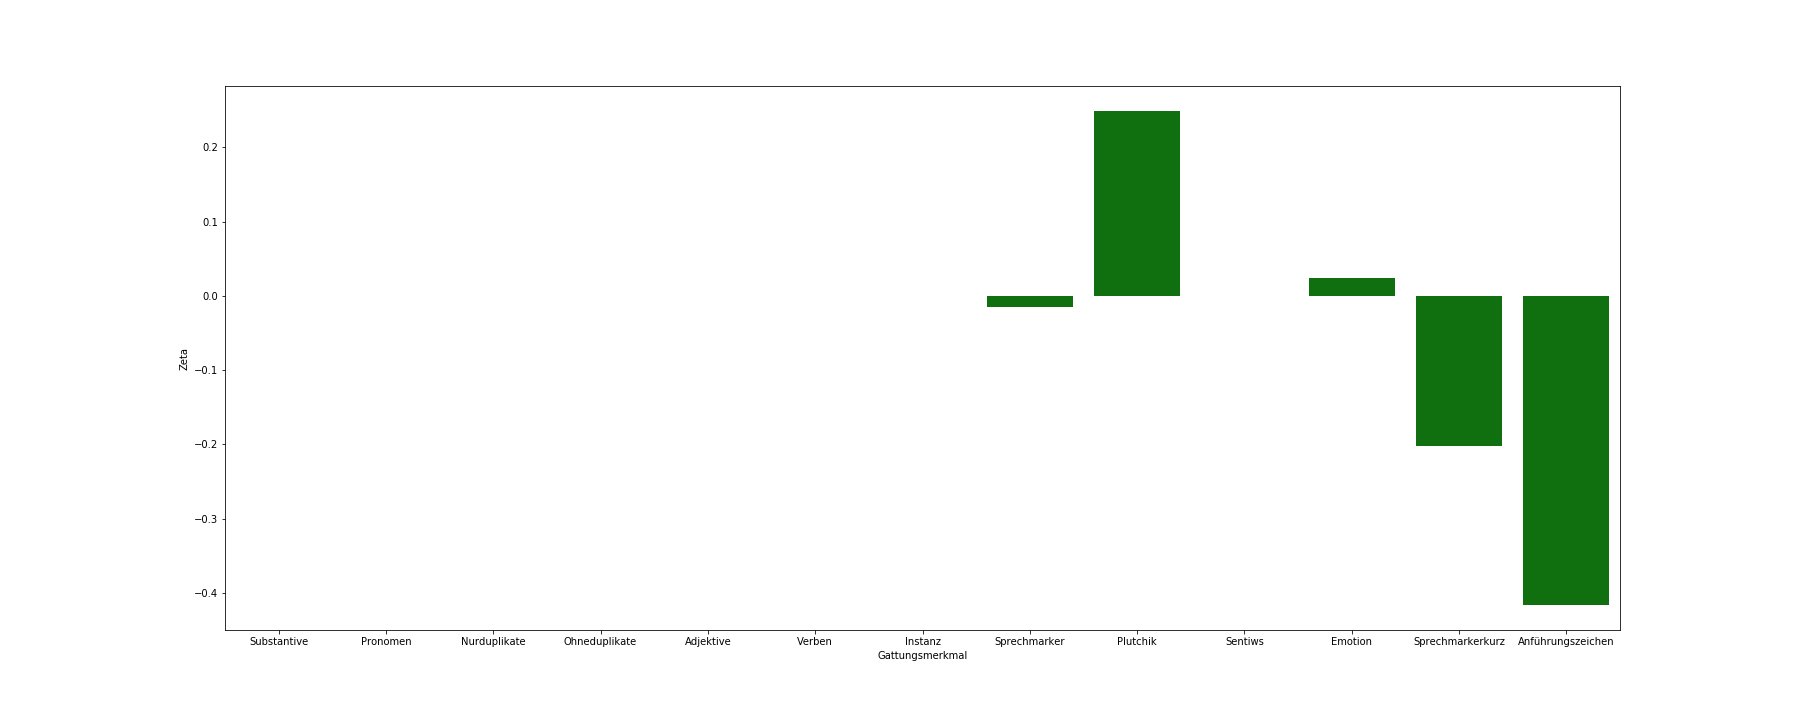
\includegraphics[width=0.5\textwidth]{haupt_alle_merkmale.png}
	\caption{Übersicht aller Merkmale und ihre allgemeine Verteilung im Hauptkorpus}
	\label{fig:haupt_alle_merkmale}
\end{wrapfigure}


Auch der Boxplot bestätigt die aufgestellten Nullhypothesen und verdeutlicht, dass eine detailliertere Untersuchung nötig ist.\\


Vergleicht man die 100 höchsten\footnote{Merkmal der Gattung Lyrik.} und niedrigsten\footnote{Merkmal der Gattung Epik.} Zetawerte der Adjektive der beiden Korpora, ist zu erkennen, dass die Verteilung der Zetawerte auf der Seite der Lyrik eindeutiger sind. Was eine leichte Tendenz der Adjektive zur Gattung Lyrik allgemein erkennen lässt. Diese Tendenz ist jedoch nicht eindeutig genug, um sie im Folgenden von den Untersuchung auf Grund eines Rauschen ausschließen zu können. Außerdem scheinen auf der Seite der Lyrik mehr emotionsbehaftete Adjektive zu liegen. \par 

Bei den Verben fällt auf, dass es sich beim eindeutigsten Verb der Epik um den Sprechmarker \textit{sagen} handelt. Doch auch hier ist auffällig, dass es in der Lyrik eindeutigere Zetawerte gibt.  \par 

Die Verteilung der Substantive zeigt, ähnlich den Adjektiven, eine Tendenz hin zur Lyrik. In beiden Fällen kann eine Untersuchung der relativen Häufigkeit sinnvoll sein. Auch eine Untersuchung der Zusammensetzung der Substantive ist sinnvoll, da es Tendenzen in Richtung Emotionswörter, Sprechmarker und Erzählung zu geben scheint.\par 

Die Untersuchung der Emotionen nach Plutchik (inklusive der Emotion \textit{Liebe}) zeigt, dass nur das Emotionswort \textit{Liebe}\footnote{die Emotion \textit{Liebe}} explizit geäußert wird. Diese explizite Emotionsäußerung kann eindeutig der Gattung Lyrik zugeordnet werden. Keine der Basisemotionen nach Plutchik weißt eindeutige Zetawerte der Gattung Epik auf. \par 

Bei der Liste \textit{Emotionen}, liegt eine deutliche Tendenz der Emotionswörter zur Gattung Lyrik vor. Insbesondere die Wörter \textit{Herz}, \textit{Seele},  \textit{Liebe} und \textit{Glück} sind mit ihren Zetawerten eindeutig. Für Epik liegen keine eindeutigen Zetawerte vor. Da die Liste der Emotionswörter allerdings sehr knapp ist, ist eine weitreichendere Untersuchung notwendig.  \par 

Eine ausführlichere Liste von Emotionswörtern wurde vom \textit{Projekt Deutscher Wortschatz} der Universität Leipzig als \textit{SentiWS} erstellt und öffentlich zugänglich gemacht. Dafür wurden die signifikantesten Nachbarschafts- und Satzkookkurenzen berechnet \citep{Sentiws}. Sie beinhaltet positive, als auch negative Wörter, die Emotionen ausdrücken und besteht aus Verben, Adjektiven und Substantiven \citep[vgl.]{Remus} Unter den 100 höchsten Zetawerten befinden sich sieben, die mit einem Wert über 0,3 eindeutig der Lyrik zugeordnet werden können. Fünfundzwanzig haben mit Werten über 0,2 eine deutliche Tendenz und cicra fünfunddreißig haben mit Werten über 0,1 eine Tendenz zur Lyrik. Auch auf Seiten der Epik finden sich keine eindeutigen Zetawerte unter -0,3. Nur fünf unter -0,2 und weisen damit eine deutliche Tendenz auf und nur circa fünfzehn weisen mit Werten unter -0,1 eine Tendenz zur Epik auf. Dies beweist eine deutliche Tendenz der Emotionswörter hin zur Lyrik auf. Aus der Graphik geht die Verteilung von Substantiven, Adjektiven und Verben jedoch nicht hervor, sodass ein Rauschen noch ausgeschlossen werden muss. \par 

Die Zetawerte der Liste \textit{Sprechmarker} verdeutlicht, dass diese deutlich der Epik zugeordnet werden können. Die Gattung der Lyrik weist keine Werte über 0,1, auf und bei den obersten Sprechmarkern handelt es sich um emotionsbehaftete Verben wie \textit{klagen} und \textit{schluchzen}. Allerdings fällt die Kategorisierung der Sprechmarker nicht so eindeutig aus wie erhofft, da auf Seiten der Epik nur \textit{sagen} mit einem Wert von -0,34 eindeutig ist. Dennoch ist eine deutliche Tendenz zu erkennen. \par 

Die genauere Untersuchung der typischen Sprechmarker in der Liste \textit{SprechmarkerKurz} zeigt, dass die gängigen Sprechmarker \textit{sagen}, \textit{fragen}, \textit{sprechen} und \textit{antworten} der Epik zugeordnet werden können. \par 

Die Untersuchung der Pronomen ergibt, dass Lyrik die Pronomen \textit{mein}, \textit{euer}, \textit{sein}, \textit{du}, \textit{unser} und \textit{wir} Tendenzen zur Lyrik aufweisen. Eine klare Aussage bezüglich der Sprecher lässt sich hieraus jedoch nicht ziehen. \par 

Die Zetawerte der Erzählinstanz zeigen keine klaren Tendenzen. \par

Da die Zetawerte lediglich angeben, wie distinktiv ein bestimmtes Wort für das Ziel- oder Vergleichskorpus steht aber noch keine Aussage darüber treffen, ob das Wort auch sehr häufig vorkommt, ist es interessant, die Positionierung einzelner Merkmale innerhalb der 100 Most Frequent Words eines Korpus zu betrachten.\par 

Die Kombination aus der Merkmalsliste der \textit{SentiWS} und der \textit{Emotionen} zeigt erwartungsgemäß auf den ersten Blick keinen eindeutigen Unterschied zwischen den beiden Gattungen. Aufgrund der Polarität der Merkmalsliste und der Tatsache, dass besonders auch implizite Emotionsausdrücke enthalten sind, sind die Wörter in beiden Gattungen nicht nur mit hohem Zetawert, sondern auch mit recht großer Häufigkeit vertreten. Dennoch ist eine Tendenz zur Lyrik erkennbar mit 27 Emotionswörtern in den 100 häufigsten Wörtern, während es bei Epik nur 18 sind. Auffällig ist, dass bei Lyrik eher beschreibende Wörter vorkommen wie \textit{schön}, \textit{dunkel} und \textit{süß}, während bei Epik mehr Verben vertreten sind wie \textit{fühlen}, \textit{wagen}, \textit{führen} und \textit{verstehen}. Insgesamt ist festzustellen, dass bei Lyrik mehr Merkmalswörter im ersten Drittel der betrachteten häufigsten Wörter vertreten sind und verschiedene Wörter in den beiden Gattungen weiter vorne liegen, dabei die Häufigkeitswerte aber in einem ähnlichen Bereich liegen. \par 

Deutlich auffälliger ist der Unterschied bei den Sprechmarkern. Während nur \textit{rufen} in den hundert häufigsten Wörtern der Lyrik vorkommt, zudem auch erst an fünfzigster Stelle, sind es bei der Epik sieben Sprechmarker. Am weitesten vorne sind \textit{rufen} und \textit{fragen} an Stelle neun und zehn, sowie etwas weiter hinten \textit{bitten} und \textit{antworten}. Hier scheinen also nicht nur die Zetawerte der Merkmalswörter, sondern auch deren Positionierung in den Most Frequent Words auf eine Zuordnung zur Epik hinzudeuten. 

Die Nullhypothese zu den Gattungsmerkmalen konnten für das Hauptkorpus bestätigt werden. Da das Korpus aber sehr unbalanciert ist und über eine große Zahl unterschiedlicher Autoren verfügt, soll im nächsten Schritt eine ausgeglichenere Textsammlung betrachtet werden.

\subparagraph{Autorenkorpus} \quad \par 

Im Vergleich zum Hauptkorpus  weist der Autorenkorpus eine allgemein ähn\-lich\-e Verteilung der Merkmale auf, die  Zetawerte sind jedoch weniger eindeutig. Da die Länge der Korpora stark unterschiedlich ist, lässt sich ein Rauschen auf Grund der Korpuslänge nicht ausschließen. Die Abgrenzung wird insbesondere auf der Seite der Lyrik weniger eindeutig. Die Tendenzen bleiben allerdings bestehen. \par 

Bei der Betrachtung der einzelnen Merkmale pro Wort fällt auf, dass die Verteilungen auf den ersten Blick identisch wirken. So bleibt die Verteilung der Zetawerte nahezu gleich, die Werte weisen allerdings Unterschiede auf. So liegen bei den Wörtern der \emph{Emotionen} Liste Zetawerte von 0,35 beziehungsweise -0,075 im Autorenkorpus vor, im Hauptkorpus liegen die Werte bei 0,4 und -0,08. Auch die jeweils eindeutigsten Wörter für Lyrik und Epik sind nahezu deckungsgleich, nur ihre Reihenfolge weicht ab. \par 

Diese Deckungsgleichheit liegt bei den Adjektiven, der Liste der Emotionen und den Substantiven  vor. Die Liste der \emph{SentiWS}-Emotionen zeigt bei den positiven Zetawerten eine identische Verteilung,  bei den negativen Werten jedoch weniger Ausreißer und Extremwerte und so eine flachere Kurve. Der Hauptkorpus hat einen größeren Bruch nach den fünf eindeutigsten Werten. Doch auch hier sind die Wörter nur durch ihre genaue Reihenfolge zu unterscheiden.  \par 

Bei der Liste der Sprechmarker sind die Werte von 0,3 und -0,4 im Gegensatz zum Hauptkorpus mit 0,1 und -0,35 im Autorenkorpus eindeutiger. Die Zetawerte im Autorenkorpus sind bei den positiven Werten der Lyrik höher und weisen hier eine größere Eindeutigkeit zu, wohingegen die Hypothese der Eindeutigkeit der Sprechmarker für Epik im Hauptkorpus eher bestätigt wird. Auch hier muss in einer weiteren Analyse das Rauschen der Korpusgröße ausgeschlossen werden. \par 

Die merkmalspezifischen Wörter und ihre Verteilung innerhalb der MFW im Autorenkorpus weicht kaum von der Verteilung innerhalb des Hauptkorpus ab, da die Verteilung der Wörter innerhalb des Merkmals kaum Differenzen aufweist. Nur die grundsätzlichen Werte der MFW weichen, vermutlich auf Grund der Korpusgröße, voneinander ab. Einzig die Cluster der \emph{SentiWS}-Emotionen in der Epik, ist im Hauptkorpus minimal klarer zu erkennen. \par 

Um den Einfluss eines einzelnen Autoren auf die Zetawerte des Hauptkorpus messen zu können und gleichzeitig das Rauschen der Korpusgröße ausschließen zu können, wird im Folgenden das Vergleichskorpus, das sich aus gemischten Texten des Hauptkorpus und Fontanetexten des Autorenkorpus zusammensetzt, untersucht. 

\subparagraph{Vergleichs- und Fontanekorpus} \quad \par 

Um die unterschiedlichen Kombinationen von Ver\-gleichs- und Fontanekorpus besser einordnen und in einen Zusammenhang setzen zu können, ist es von Interesse zunächst die Zetaergebnisse für jedes allein für sich stehende Korpus zu betrachten. Wirft man zunächst erneut einen Blick auf den gesamten Zetawert pro Merkmalsliste für das Vergleichskorpus, weisen besonders Plutchiks Emotionswörter mit einem Wert von 0,3  deutliche Tendenzen in Richtung lyrischer Texte auf. Die daraus erweiterte Emotionswortliste erreicht hingegen nur kaum einen Zetawert über 0, während \textit{SentiWS} ebenfalls neutral bei 0 bleibt. Deutlich als Merkmal für Epik sprechen Anführungszeichen. Diese Beobachtungen stimmen erwartungsgemäß in etwa mit den Ergebnissen des Hauptkorpus überein, aus dem das Vergleichskorpus gesamplet wurde.

Die Gegenüberstellung mit denselben Werten für das Fontanekorpus ist besonders interessant. Auch hier weisen die Merkmale von Plutchik und die Anführungszeichen die höchsten Zetawerte auf, während die Sprechmarker wie oben nur leicht Richtung Epik ausschlagen. Hier ist allerdings die Skalierung der Werte zu beachten: Im Vergleichskorpus erlangen Anführungszeichen ein Zeta von -0,4, bei Fontane hingegen nur -0,06. Obwohl also die autorspezifische Verwendung der Merkmale vergleichbar mit deren Anteil im Vergleichskorpus ist, sind die Werte verschwindend klein. Das kann entweder darauf zurückzuführen sein, dass Fontane beispielsweise Plutchiks Emotionen im Vergleich zum Hauptkorpus überdurchschnittlich häufig in der Epik verwendet, was zu einer nur sehr leichten Tendenz Richtung Lyrik führt. Es ist aber auch möglich, dass die jeweiligen Merkmale in nur wenigen Segmenten, dafür aber tendenziell eher in einer der Gattungen verwendet sind. Da die erweiterte Hypothese der vorliegenden Arbeit davon ausgeht, dass das Autorschaftssignal soweit reduziert werden kann, dass eine stilometrische Unterscheidung der Gattungen davon unbeeinflusst ist, werden verschiedene Kombinationen der Korpora auf dieselben Merkmale hin untersucht. \par 

Zunächst wird das Vergleichskorpus nur mit den Epiksegmenten von Fontane angereichert. Die auffälligen Merkmale sind auch hier wieder dieselben. Der Wert für Plutchiks Emotionen ebenso wie die Sprechmarker sind unverändert, während die Anführungszeichen statt leicht über -0,4 nun etwas darunter liegen. Werden Fontanes Lyriksegmente zum reinen Vergleichskorpus hinzugefügt, ist eine etwas stärkere Veränderung zu beobachten. Plutchiks Emotionen liegen nun etwas unter Zeta von 0,3, während sie davor leicht darüber lagen. Das ist möglicherweise damit zu erklären, dass entsprechend dem Zetawert anteilig ein geringerer Prozentsatz der Segmente bei Fontane, nur etwa 5 Prozent, die analysierten Emotionswörter enthalten, während diese im Vergleichskorpus in etwa 30 Prozent der Segmente zu finden sind. In Kombination der beiden Korpora muss damit also der entsprechende Werte sinken. Auch bei den Anführungszeichen ist eine ähnliche Beobachtung zu machen. Betrachtet man nun die Merkmalswerte für eine Kombinationen der beiden kompletten Korpora ergibt sich erneut ein ähnliches Bild. Auch hier sind die Werte für Plutchik und die Anführungszeichen leicht Richtung 0 gewandert, für die anderen Merkmale ist keine signifikante Veränderung zu erkennen. Insgesamt scheint also das Hinzufügen und Entfernen eines Autors aus einem Korpus nur die Höhe der Werte leicht zu modifizieren, schlussendlich aber keinen signifikanten Einfluss auf die allgemeine Verteilung zu haben. \par 

Ein genaueres Verständnis hierfür gibt ein Blick auf die einzelnen Wörter der Merkmalslisten. Hier erklärt sich, warum der gesamte Zetawert für Plutchiks Emotionen besonders in Richtung Lyrik ausschlägt. Drei der neun Wörter, \textit{Liebe}, \textit{Freude} und \textit{Trauer} haben eindeutig positive Werte, wobei ersteres den deutlich größten Wert von 0,35 im Vergleich zum Nachfolger mit 0,15 hat. Nur drei Wörter weisen negative Werte auf, die minimal unter 0 liegen. Ein Großteil der Merkmalsliste spricht also für Lyrik. Im Vergleich dazu wird damit auch der neutrale Gesamtzetawert für die Emotions- und Sprechmarkerliste deutlich. Zwar gibt es jeweils einige Wörter, die eine eindeutige Tendenz zu einer Gattung haben, z.B. \textit{singen} mit 0,35 vs. \textit{sagen} mit -0,32. Insgesamt ist die Verteilung der Zetawerte im positiven und negativen Wertebereich aber in etwa ausgeglichen, was eine Neutralisierung des Gesamtwertes erklärt. \par 

Für das Korpus mit allen Vergleichs- und Fontanetexten ist insgesamt eine vergleichbare Verteilung zu beobachten. Auch hier sind die Merkmale mit neutralen Gesamtwerten gleichmäßig auf positiv und negative Einzelwerte verteilt, während bei Plutchik ein Großteil der Wörter in Richtung Lyrik tendiert. Auch die spezifischen Wörter mit den höchsten Zetas sind beinahe unverändert und haben teilweise nur ihre Position vertauscht. \textit{Liebe} ist weiterhin an erster Position, hat aber einen leicht niedrigeren Wert mit 0,3 statt 0,35. Auch bei den Sprechmarkern zeigt sich ein ähnliches Bild, \textit{singen} spricht weiter am stärksten für Lyrik mit 0,37, während \textit{sagen} sogar mit noch eindeutigerem Wert von -0,42 als episches Merkmal eingestuft wird. \par 

Stellt man diese Werte nun mit dem Fontanekorpus gegenüber wird der Einfluss des Autors auf das kombinierte Korpus deutlich. Der Sprechmarker \textit{sagen} weist hier einen sehr eindeutigen Wert von -0,65 Richtung Epik auf. Bei Plutchiks Emotionen hingegen ist beispielsweise \textit{Wut} das Wort mit dem zweitgrößten Zeta. Während es bei Fontane also eher in Lyriktexten auftritt, hat dies keinen Einfluss auf die Kombination mit dem Vergleichskorpus. \par 


Besonders große Zetawerte eines einzelnen Autors scheinen also Einfluss auf das Gesamtergebnis zu nehmen, während kleinere Werte eher in den restlichen Werten untergehen. Gleichzeitig wird aber trotz einer Veränderung der Zetawerte deren insgesamte Verteilung und Tendenz nicht verändert. Zudem wurde mit den Fontanesegmenten eine sehr große Zahl von Texten eines einzelnen Autors hinzugefügt, wodurch das Vergleichskorpus um fast das Eineinhalbfache vergrößert und damit ein signifikanter Einfluss auf die Zusammensetzung des Korpus genommen wurde. \par 

Auch hier ist es wieder von Interesse, die Positionierung der Merkmale innerhalb der Most Frequent Words zu betrachten. In der Lyrik des Vergleichskorpus liegen 28 Wörter aus \textit{SentiWS} und \textit{Emotionen} innerhalb der 100 häufigsten Wörter, während es bei Epik nur 14 sind. Zwar überschneidet sich die Reihenfolge der Wörter etwas, \textit{Herz} ist das erste gefolgt von \textit{schön}, allerdings ist ersteres in der Lyrik bereits das dritthäufigste Wort, in der Epik hingegen erst das dreiundzwanzigste. Bei den Sprechmarkern ist ein ähnliches, nur umgekehrtes Bild zu beobachten. Nur zwei sind in den MFW der Lyrik vertreten, wobei das emotionsbetonte \textit{singen} das häufigste ist. In der Epik hingegen sind acht Sprechmarker auch häufig verwendet. Wie bereits mehrfach beobachtet, liegen auch hier \textit{fragen} und \textit{rufen} vorne. Diese beiden Merkmale scheinen also recht zuverlässig für die jeweilige Gattung zu sprechen. \par 

Im Vergleichskorpus mit Fontanes Epiktexten ist eine sehr ähnliche Beobachtung zu machen, auch hier sind in Epik mehr Sprechmarker, in der Lyrik mehr Emotionen zu verzeichnen. Sogar die häufigsten Merkmale überschneiden sich. So sind erneut \textit{fragen} und \textit{rufen} die häufigsten Redeeinleitungen in der Epik, während \textit{herz} und \textit{schön} in beiden Gattungen die häufigsten der Emotionswörter sind. Lediglich \textit{alt} erscheint bei der Epik nun an erster Stelle, was wiederum auf den Einfluss von Fontanes Epik zurückzuführen ist. Auch dort ist das Wort an siebter Stelle der häufigsten Wörter zu finden und ist damit von sechsundzwanzigster Stelle im reinen Vergleichskorpus auf die neunte im kombinierten Korpus gesprungen. Werden statt der Epik die Lyriktexte hinzugefügt, ist kaum eine Veränderung zu verzeichnen. Darauf weisen bereits die Ergebnisse weiter oben hin, in denen deutlich wurde, dass Fontanes Gedichte weniger von denen des Vergleichskorpus abweichen als der Roman. \par 

Infolge dieser einzelnen Kombinationsbeobachtungen, zeigen auch die Ergebnisse für das Vergleichskorpus vermischt mit dem Fontanekorpus ähnliche Verteilungen. Erneut ist \textit{alt} das häufigste Emotionswort in der Epik, was wieder auf den Einfluss von Fontanes Roman hinweist. Da es sich hierbei um \textit{Mathilde Möhring} handelt, ist ein übermäßiger Gebrauch des Wortes eventuell daraufhin zurückzuführen. Auch die Sprechmarker sind vergleichbar wie oben verteilt. \par 

Die vorangegangenen Berechnungen haben ergeben, dass über alle Korpora hinweg Emotionen sowohl eindeutiger, als auch häufiger in Texten der Gattung Lyrik zu finden sind. Die eindeutigsten Zetawerte der Emotionen werden mit der Merkmalsliste von Plutchik erzielt, die im Gegensatz zu den anderen Emotionslisten ausschließlich explizite Emotionen enthält. Die Auswertung der Zetawerte der Erzählinstanz hat aufgrund des Aufbaus des Merkmals keine Ergebnisse geliefert, da Pronomen sich als ungeeignetes Mittel erwiesen haben. Generell eignen sich semantische Merkmale nicht zur Definition der Erzählinstanz. Für eine erfolgreiche Merkmalsanalyse muss ein Vefahren gewählt werden, das die syntaktische Struktur eines Textes berücksichtigt. Neben den eindeutig epischen Anführungszeichen der direkten Rede wird auch die indirekte Rede anhand der vorher definierten Sprechmarker eindeutiger und häufiger der Epik zugeordnet. Insgesamt konnten die zuvor aufgestellten Hypothesen zu den inhaltlichen Gattungsmerkmalen, bis auf die Sprechinstanz, bestätigt werden. Unabhängig vom Korpusaufbau sind die Zetawerte der Merkmale ähnlich verteilt. Bezüglich Fontanes Autorsignals im Vergleichskorpus ist festzustellen, dass die Zetawerte des Lyrikkorpus inklusive Fontane eine noch geringere Abweichung vom Vergleichskorpus aufweisen als die des Epikkorpus inklusive Fontane. Dieses Phänomen lässt sich vermutlich auf ein leichtes Rauschen bezüglich des spezifischen Romans zurückführen. Eine Lösung ist möglicherweise der Gegentest mit einem weiteren Autor oder einem anderen Roman. Ein Rauschen durch ein Autorsignal soll im Folgenden mit der Berechnung der Deltawerte ausgeschlossen werden.


\subsection{Delta - Resultate}

Die Berechnung der Deltas wird zunächst mit dem Autorenkorpus durchgeführt. Um ein erstes Verständnis für die Ergebnisse zu erlangen, ist eine Visualisierung der Normalverteilung der Deltawerte hilfreich. Die dunklere Kurve, mit \textit{different} annotiert, gibt an, dass der abgebildete Deltawert das Resultat der Gegenüberstellung zweier Texte unterschiedlicher Gattung ist. Die hellere \textit{same}-Kurve steht umgekehrt für Datenpaare derselben Gattung. Beim Vergleich eines Lyrik- und eines Epiktextes fällt ein eindeutiger Peak bei 0 auf sowie eine steil abfallende Kurve, die sich innerhalb eines Wertebereichs von -0,2 und 0,2 für das Cosinusdelta bewegt. Die Kurve für Texte derselben Gattung ist hingegen sehr unregelmäßig, weist bei 0 ein Minimum auf und hat mehrere kleinere Peaks. Dabei bewegt sich ein Großteil der Kurve allerdings im selben Wertebereich wie die \textit{different}-Kurve \footnote{Der deutlich höhere Count für Deltawerte bei 0 für die \textit{different}-Kurve ist mit der großen Anzahl Texte, die analysiert werden, zu erklären. Jeder Text wird für das Delta mit jedem gegenübergestellt, weshalb deutlich häufiger das Label \glqq different \grqq vermerkt wird.}. Die grau schraffierte Fläche zeigt die Überschneidung der beiden Kurven an, die für eine erfolgreiche stilometrische Analyse möglichst gering sein sollte. Da hier die Schnittfläche aber zeigt, dass die Deltawerte sowohl für Datenpaare derselben als auch verschiedener Gattung fast identisch sind und keine klare Tendenz aufweisen. Das deutet darauf hin, dass eine Unterscheidung mithilfe von Deltaberechnungen für dieses Korpus eher ungeeignet ist. \par 

Bevor diese Annahme bestätigt werden kann, müssen weitere Faktoren beachtet werden. Als Grundlage für das Delta dienen Z-Scores, die angeben, wie stark die Verwendung eines Wortes in einem Text im Verhältnis zu dessen Verwendung im gesamten Korpus abweicht. Sie werden zunächst für alle Wörter berechnet und dann abgeschnitten. In diesem Fall werden nur die 1000 häufigsten Wörter verwendet, die eine gesamten Wertespanne der Z-Scores zwischen -0,6 und 49 ergeben. Die unterdurchschnittliche Verwendung von Wörtern weicht also kaum vom Mittel ab, während andere in bestimmten Texten signifikant häufiger als im restlichen Korpus zu verzeichnen sind. \par 

Für die vorliegende Arbeit sind die Wörter am interessantesten, die Teil der Gattungsmerkmale sind. Hierfür wird für jede Gattung der Durchschnitt der Z-Scores pro Wort gebildet. Von den Emotionswörtern sind 35 auch in den Z-Scores zu finden. Fast alle Werte liegen für Epiktexte im negativen Bereich, was bedeutet, dass die entsprechenden Wörter unterdurchschnittlich häufig verwendet werden. Den kleinsten Wert mit -0,3 weist dabei \textit{Herz} auf. Im Zusammenhang mit dem Wertebereich der Z-Scores zeigt sich, dass das Wort verhältnismäßig stark im Negativen liegt. Die positiven Werte sind dagegen mit maximal 0,1 im Vergleich zum Maximum von 49 sehr klein und sprechen kaum dafür, dass sie typischerweise in Epiktexten verwendet werden. Dennoch ist interessant, dass teilweise dieselben Wörter, die bei den Zetaanalysen als spezifisch für Epik erkannt wurden, auch hier im positiven Wertebereich liegen: \textit{Vertrauen} und \textit{Freude}. Ein Problem ist aber, dass die Emotionswörter für Lyriktexte nicht erkennbar sind, die meisten Werte betragen 0 oder sind minimal. Möglicherweise ist diese Beobachtung darin begründet, dass deutlich mehr lyrische Texte im Korpus sind, damit großen Einfluss auf die mittlere Verwendung von Wörtern haben und dadurch nicht stark von diesem Mittel abweichen. \par 

Bei der Untersuchung der Sprechmarker hingegen zeigt sich ein deutlicheres Bild. Die beim Zeta bereits als distinktiv epische Verben identifizierten Wörter wie \textit{antworten, bemerken, berichten, rufen} weisen auch bei den Z-Scores negative Werte für die Lyriktexte auf, werden dort also seltener als im Durchschnitt verwendet. Umgekehrt ist auch hier \textit{singen} als Wort erkannt, das in der Lyrik überdurchschnittlicher verwendet wird als im Epikkorpus - dort ist der Wert für das Wort deutlich negativ. Sowohl für Emotionen als auch für die Sprechmarker ist insgesamt festzustellen, dass die Z-Scores sich in eher kleinen Wertebereichen bewegen. Dabei muss aber beachtet werden, dass die kleinen Z-Scores deutlich häufiger auftreten als die sehr großen, also nur sehr wenige Wörter extrem über der durchschnittlichen Verwendung liegen. Damit sind also auch kleinere Werte aussagekräftig. \par 

Insgesamt scheint das Delta-Verfahren für das Autorenkorpus aber eher ungeeignet zu sein. Gründe dafür sind möglicherweise, dass zu viele Lyriktexte im Verhältnis zur Epik enthalten sind und deshalb zu viel Einfluss auf die Werte nehmen. Gleichzeitig beeinflussen möglicherweise aber auch die Textlängen die Resultate, da die Z-Scores für die kompletten Texte berechnet werden und erst dann entsprechend des gewählten MFW-Levels abgeschnitten werden. Obwohl dieser Wert hier bei 1000 gewählt wurde, um ein Mittelmaß zwischen kurzen Gedichten und langen Romanen zu finden, kann dennoch nicht die starke Varianz zwischen extrem kurzen und langen Dokumenten berücksichtigt werden. Ein Ansatz, dieser Schwierigkeit entgegen zu wirken, ist, das Delta-Verfahren auf die im Zeta verwendeten Segmente, statt den tatsächlichen Texten anzuwenden. Möglicherweise kann dadurch auch wie bereits im Zeta das Autorensignal zumindest etwas relativiert werden. \par                 

Bei der Betrachtung der \textit{same-} und  \textit{different-}Kurve zeigt sich ein ähnliches Bild wie bei den Originaltexten. Auch hier überschneiden sich beide Kurven fast komplett mit einem Peak jeweils um 0. Lediglich die Darstellung der Werte für Segmente derselben Gattung ist regelmäßiger und hat nur noch ein Maximum. Auch hier befindet sich ein Großteil der Cosinuswerte in einem Bereich von -0,1 und 0,2, während größere Werte nur sehr selten berechnet werden. Obwohl diese Betrachtung der Resultate sehr ähnlich zu der oben besprochenen Analyse ist, weisen die Z-Scores der Gattungsmerkmale deutlichere Ergebnisse auf. Bei den Emotionsmarkern treten Wörter wie \textit{Herz} und \textit{Seele} überdurchschnittlich häufig in der Lyrik auf, während beispielsweise \textit{ängstlich} und \textit{schämen} eher für Epiksegmente verzeichnet sind. Auch hier zeigen sich wieder Parallelen zu den vorherigen Zeta-Analysen. Besonders ins Auge sticht jedes Mal \textit{Herz} mit auffällig hohen Werten, wie hier mit 0,4 in Richtung der Lyrik. \par 

Während bei den Emotionswörter kaum extreme Ausreißer erkennbar sind und sich die Z-Score-Werte recht nah um 0 bewegen, sind bei den Sprechmarkern deutlichere Tendenzen zu beobachten. Wie bereits mehrmals ist auch hier \textit{singen} ein Wort, das deutlich auf einen lyrischen Text hinweist. Äquivalent dazu sind in den epischen Segmenten \textit{antworten}, \textit{bemerken}, \textit{bitten} und \textit{rufen} überdurchschnittlich häufig verwendet und umgekehrt in den Lyriksegmenten entsprechend seltener. \par 

Vergleicht man nun die 100 größten Cosinus-Werte für das rohe Autorenkorpus und für dessen Segmentaufbau, zeigen sich deutliche Unterschiede. Entsprechend einer Einfärbung nach Gattungen sind alle Texte mit nahe beieinander liegenden Deltawerten der Lyrik zugeordnet, während bei den Segmenten zweimal Lyrik ähnliche Werte wie die Epik erhalten hat. Auffällig ist, dass bei den Texten Lyrik die kürzesten Distanzmaße aufweist, während es bei den Segmenten fast nur Epiktexte in den 100 kleinsten Distanzen vertreten ist. Das ist möglicherweise damit zu erklären, dass im grundlegenden Korpus die Anzahl der Gedichte deutlich überwiegt und damit das Mittel stärker beeinflusst als bei den ausgeglichenen Segmenten. \par 

Noch deutlicher wird der Unterschied zwischen rohen Texten und Segmenten, wenn als Distanzmaß die Manhattan-Distanz statt des Cosinus-Maßes verwendet wird. Während bei den ursprünglichen Texten weiterhin alle Dokumente mit geringer Distanz zueinander nur einer Gattung zuzuordnen sind, entsteht bei den Segmenten ein gemischteres Bild. Zwar können teilweise einige Segmente mit ähnlichem Distanzwert einer Gattung zugeordnet werden. Diese Manhattenwerte liegen aber so nah an denen der anderen Gattung, dass keine klare Unterscheidung möglich ist. Durch die Segmentierung geht also wohl zu viel Information verloren. Betrachtet man schließlich für das Korpus mit den Gesamttexten die Zuordnung zu Autoren, zeigt sich wiederum ein ungleichmäßiges Bild. Das Autorsignal kann nicht vollständig eliminiert werden, immer wieder sind Texte eines Autors aufgrund des Cosinuswertes zusammen gruppiert. Besonders Kellers Gedichte scheinen einander sehr ähnlich zu sein. Da aber dennoch immer auch die gleiche Gattung gemeinsam gruppiert wird, kann angenommen werden, dass das Autorsignal zwar nicht komplett herausgefiltert werden kann, aber keinen so signifikanten Einfluss auf die stilometrischen Ergebnisse hat, dass eine Gattungszuordnung nicht mehr möglich wäre. Im Folgenden wird überprüft, ob diese Beobachtung nur für einzelne Korpora gilt oder ob die Annahme haltbar ist. Zudem muss beachtet werden, dass hier nur die 100 höchsten Deltawerte, die nahe an 1 liegen und damit eine sehr große Ähnlichkeit zwischen den beiden gemeinsam analysierten Texten ausdrücken, betrachtet wurden. Am Ende dieses Kapitels soll diese Beobachtung noch erweitert werden. \par 

Um die Ergebnisse besser generalisieren zu können, wird dieselbe Analyse auf für das Vergleichskorpus durchgeführt. Die \textit{same-} und  \textit{different-}Kurven liegen erneut übereinander, sodass keine klare Differenzierung möglich ist, und sind um 0 zentriert. Die \textit{different}-Kurve weist einen zweiten kleinen Peak auf. In Gegenüberstellung mit der Visualisierung der Kurve für das Fontane-Korpus, das Teil des Vergleichskorpus ist, wird ersichtlich, dass auch dort ein Peak an ähnlicher Stelle zu erkennen ist, was auf einen möglichen Einfluss von Fontanes Texten zurückzuführen ist. \par 

Auch die Analyse der Z-Scores für die Gattungsmerkmale ist vergleichbar mit den Ergebnissen für das Autorenkorpus. Nicht nur die Wörter, die besonders für Lyrik und Epik sprechen, sind ähnlich oder sogar dieselben, auch die zugehörigen Werte sind kaum verändert. So ist \textit{Herz} erneut das unterdurchschnittlichste Emotionswort für Epiktexte mit einem Wert von -0,33. Ebenso ist bei den Sprechmarker \textit{singen} erneut das ausschlaggebendste Wort für Lyrik, während \textit{bitten} und \textit{erzählen} häufiger als das Mittel in Epiktexten verwendet werden. Auffällig bei letzterem Wort ist, dass es einen deutlich größeren Z-Score in Richtung der Epik aufweist als in der vorhergehenden Analyse. Ein Blick auf den Wert bei Fontane gibt aber auch hier wieder Aufschluss. Nur vier Wörter erlangen bei ihm einen positiven Z-Score, wobei drei kaum über 0 liegen. \textit{erzählen} hingegen ist ein deutlicher Ausreißer, der wiederum das gesamte Korpus zu beeinflussen scheint. \par 

Der große Anteil von Fontanes Texten hat also wie zu erwarten im Bereich der Z-Scores deutlich erkennbaren Einfluss auf die Deltaanalyse des Vergleichskorpus. Die 100 größten Cosinus-Werte hingegen scheinen recht robust gegen diese unbalancierte Zusammenstellung zu sein. Zwar ist eine signifikante Anzahl an Texten von Fontane vertreten und teilweise auf zusammen gruppiert. Die Hälfte dieser 100 ähnlichsten Texte stammt allerdings von unterschiedlichen Autoren, wobei es sich zudem durchgehend um Gedichte handelt. Auch hier funktioniert die Manhattan-Distanz ebenso gut die das Cosinus-Maß. Wirft man noch einen Blick auf die Delta-Analyse mit den Segmenten des Vergleichskorpus, wird eine Parallele deutlich. Auch hier weisen Epiksegmente die höchsten Delta-Werte auf. Dieses Mal sind allerdings keine Gedichte bei diesen geringsten Distanzen zu verzeichnen, was eine sauberere Zuordnung ermöglichen kann. \par 

Anstatt nur vereinzelte Werte zu betrachten, ist ein Überblick über verschiedene Korpora und ihre allgemeinen Ergebnisse hilfreich für eine Einschätzung der Qualität der stilometrischen Untersuchung. Aus diesem Grund soll der Anteil der richtig eingeordneten gegenübergestellten Textpaare berechnet werden, deren Cosinus-Wert über einem Cutoff-Wert von 0,35 \footnote{Dieser Wert wurde in einer anderen Projektarbeit berechnet und getestet.} liegt und die damit derselben Gattung zugeordnet werden. Für das Autoren- und das Fontanekorpus werden auf Basis des Cosinuswertes alle Dokumentpaare oberhalb des Cutoffs richtigerweise derselben Gattung ebenso wie demselben Autor zugeordnet. Wie bereits oben festgestellt, ist die Verwendung der Segmente ungeeignet für eine Deltaanalyse. Im Autorenkorpus ist der Anteil von richtig und falsch zugeordneten Gattungen fast ausgeglichen, während im Vergleichskorpus mit Fontanetexten die Zahl der falsch zugewiesenen Gattungsbezeichnungen deutlich überwiegt. Bei der Verwendung dieses Korpus mit den originalen Texten hingegen zeigt sich ein anderes Bild. Die Autorschaft wird zwar nur unzufriedenstellend erkannt, was aber außer Acht gelassen werden kann, da das Autorensignal ohnehin herausgefiltert werden soll. Die Gattungszuordnung ergibt hingegen bessere Ergebnisse. Nur ein geringfügiger Anteil der analysierten Textpaare wird einer falschen Gattung zugewiesen. \par 

Obwohl diese Resultate zunächst zufriedenstellend wirken, muss der geringfügige Anteil der Cosinus-Werte die über dem Cutoff liegen beachtet werden. Von insgesamt 9.843.834 verglichenen Dokumentpaaren im Vergleichskorpus liegen nur 2.200 Deltawerte über 0,35, wovon 50 falsch einsortiert werden. Bereits die \textit{same- und different}-Kurven vom Beginn des Kapitels haben auf diese Beobachtung hingewiesen. Ein signifikanter Großteil der Daten liegt zwischen etwa -0,2 und 0,2 und ist nur schwer einer bestimmten Gattung zuzuordnen, während wenige Werte über diesem Bereich liegen und dafür nahezu perfekt einzuordnen sind. Dadurch bietet sich die Möglichkeit, den Cutoff zu verkleinern und auf 0,2 zu setzen. Tatsächlich ist dies erfolgreich. Beim Vergleichskorpus werden nun bereits 23.044 Textpaare richtig zugewiesen und nur 216 falsch klassifiziert. Dennoch handelt es sich um einen Anteil, der für eine Attribution im realen Anwendungsfall nicht zuverlässig genug ist. Da das Verfahren für die Gattungszuweisung allerdings dennoch in Teilen funktioniert, wäre ein weiterer Ansatzpunkt ein modifizierter Korpusaufbau. Ein ausgeglicheneres Verhältnis von Epiktexten, möglicherweise nur mit Sampleausschnitten daraus, und Gedichten könnte die Ergebnisse verbessern. Ebenso könnte es von Bedeutung sein, mehr darauf zu achten, dass das Vorkommen von Autoren balancierter ist und nicht wie beispielsweise im Vergleichskorpus ein Autor beinahe ein Drittel des gesamten Korpus ausmacht.


\subsection{Fazit}
Die Ergebnisse, die durch das Zeta- bzw. Deltaverfahren gewonnen werden konnten, zeigen, dass eine computergestützte Gattungsattribution anhand inhaltlicher Merkmale zufriedenstellende Resultate liefern kann. Im Besonderen hat sich dabei herauskristallisiert, dass die Analyse nach Emotionen und Sprechsituationen eine klare Abgrenzung der Gattungen ermöglicht. Diese Beobachtung konnte durch die Arbeit mit unterschiedlich aufgebauten Korpora gestützt werden, wobei Rauschsignale wie Korpusgröße, Balanciertheit und Autorschaft nach und nach reduziert und ausgeschlossen werden konnten. Weiterhin fällt auf, dass epische Texte eine größere Wortvarianz aufweisen, sodass auch eine merkmalsunspezifische Aufteilung nach Lyrik und Epik möglich ist. Diese Wortvarianz verstärkt die Distinktivität der Gattungsmerkmale. Auf Seiten der Epik haben sich somit viele Elemente einer Merkmalsliste (\textit{Sprechmarker}) gegen das hohe Aufkommen alternativer Wörter durchgesetzt, obwohl eine gleichmäßigere Verteilung zu erwarten wäre, wohingegen der lyrische Wortschatz eher von Emotionen geprägt ist. \par 

Nicht nur die Eindeutigkeit der mittelfrequentierten Wörter der Zetaanalyse, auch durch die Deltaanalyse mithilfe der häufigsten Wörter konnte bewiesen werden, dass bei entsprechendem Korpusaufbau das Autorschaftssignal so weit reduziert werden kann bzw. an Bedeutung verliert, dass eine Zuordnung nach Gattungen erfolgreich möglich ist. Daraus lässt sich schließen, dass auch mit weiteren stilometrischen Methoden eine inhaltsbasierte Gattungsattribution erfolgsversprechend ist. \par 

Neben den oben aufgeführten Varianzen innerhalb des Korpusaufbaus bietet es sich für kommende Analysen an, weitere Parameter zu verändern. Beispielsweise wäre es von Interesse, herauszufinden, ob eine Gattungszuordnung nur innerhalb einer Epoche oder auch epochenübergreifend und somit allgemeingültig vonstatten gehen kann. Auch eine automatisierte Gattungszuweisung mithilfe von aus den Ergebnissen berechneter Cutoffwerte für neue, ungesehene Korpora erscheint wissenswert. Außerdem könnte auch eine Gegenüberstellung mit Dramen erfolgen.






\section{Bibliographie}
\bibliographystyle{apalike}
\bibliography{/home/teresa/Dokumente/Stilometrie}
\end{document}
